% =====================================================================
% ARR submission: the comprehension-screen evaluation paper.
%
% Every number below is regenerated by a script, never typed from memory:
%   results/derived/arr_transfer/report.md         (17-route and 3-family results)
%   results/derived/arr_screen_baselines/report.md (9-route v6 baselines)
%   results/frontier/admission_campaign{,_v5,_v6}  (retest table)
%   results/frontier/baseline_campaign_v6/derived/audit_versus_behaviour.json
% Preregistration: docs/arr-transfer-campaign-prereg-2026-09-19.md.
%
% Template: official ACL style files, unmodified. Keep [review] until
% acceptance. Build: pdflatex, bibtex, pdflatex, pdflatex.
% =====================================================================

\documentclass[11pt]{article}

\usepackage[review]{acl}

% Local toolchain only: the lineno shipped here places right-column numbers
% inside the left column; pin them left of each column. acl.sty is untouched.
\makeatletter
\@ifpackageloaded{lineno}{%
  \leftlinenumbers*
  \setlength{\linenumbersep}{4pt}%
  \renewcommand\linenumberfont{\normalfont\tiny\sffamily\color{lightgray}}%
}{}
\makeatother

\usepackage{times}
\usepackage{latexsym}
\usepackage[T1]{fontenc}
\usepackage[utf8]{inputenc}
\usepackage{microtype}
\usepackage{graphicx}
\usepackage{booktabs}
\usepackage{url}

\title{Who Passes Depends on the Questions:\\
       Validity Evidence for the Comprehension Screens\\
       that Admit Language-Model Agents to Strategic Studies}

\author{Anonymous ARR submission}

\begin{document}
\maketitle

\begin{abstract}
Studies that read language-model behaviour as strategy increasingly admit a
model only after it passes a comprehension screen: a fixed set of questions
about the game, scored against ground truth. The screen selects the sample
every later claim is about, yet it is rarely treated as a measuring
instrument. We test one screen the way an instrument is tested, and we build
two more for games whose state has a different shape: an iterated social
dilemma, where the opponent's history must be tracked, and a four-player public
goods game, where an aggregate must be tracked. Of 24 preregistered hosted
endpoints, 17 produced complete answers. Three findings follow.
The screen is repeatable and it is not a proxy for the model's name: on nine
endpoints the name reproduced the verdict exactly, but on 17 five endpoints
break that rule. Endpoint rankings transfer across the three games, with rank
correlations of 0.66 to 0.87 on overall accuracy. Verdicts do not: the same
thresholds admit 8 of 17 endpoints in the first game, 1 of 17 in the second
and none of 16 in the third. In exploratory analysis, how many numbers an
answer must combine explains much of the item difficulty ($\rho=-0.74$ over 60
items). A screen's admit set is therefore a property of its questions as much
as of the agent. We give the checks a screening study should report.
\end{abstract}

% =====================================================================
\section{Introduction}
\label{sec:intro}

A behavioural study of language-model agents first has to decide which models
it is about. More and more often the decision is made by a comprehension
screen. Before any choice is read as strategy, the model answers questions
about the rules and the state of the game, the answers are scored against
ground truth, and only models above a threshold enter the analysis
\citep{huang2026probing,cacioli2026screen}. The reason is sound. A move that
parses is not evidence that the agent followed the game, and human experiments
have long gated participants on exactly this kind of check
\citep{oppenheimer2009instructional,chou2009control}. In the most cited study
of language models in repeated games, the human participants had to answer a
comprehension questionnaire before they could play, while the models did not
\citep{akata2025playing}.

A screen is two things at once. It is a measuring instrument, and it is a
selection rule on the sample that every later claim is made about. Whatever
the screen fails to measure, the study inherits, and whatever the screen is
accidentally correlated with, the study's sample is selected on. The human
literature learned this the hard way: passing an attention screener correlates
with respondent characteristics, so dropping failers changes who the results
describe \citep{berinsky2014separating,aronow2019note}. The same question has
not been asked of the screens used for models.

We ask it. We take a frozen screen of twenty questions over six domains, used
to admit hosted language-model endpoints to a study of a repeated two-player
race, and put it through the tests an instrument gets
\citep{wallach2025position,salaudeen2025measurement}. Is it repeatable? Does it
carry information that a free signal such as the model's name does not? And
does a score earned on one game describe the same agent on another game? For
the last question we built two further screens with identical structure, for
games whose state has a different shape, and administered all three to the same
roster under a preregistered plan.

The answer has two halves, and the paper is about the gap between them. The
screen measures something real. It is repeatable, a model's name does not
reproduce its verdict once the roster is wide enough, and endpoints that rank
high on one game rank high on the others. But the verdict does not travel. At
identical thresholds the first game admits eight of 17 endpoints, the second
admits one and the third admits none. The items explain why. How many numbers a
correct answer has to combine predicts much of an item's difficulty, and the
new games ask for longer sums. An admit set is therefore partly a
property of the questions, so the sentence ``the model understood the game''
needs the questions attached to it.

Our contributions are:
\begin{itemize}
\item A preregistered validity study of a comprehension screen for
      language-model agents, covering structure, repeatability, discriminant
      validity against cheap signals and transfer across three task families
      (\S\ref{sec:design}, \S\ref{sec:results}).
\item Evidence that a tie between the model name and the verdict, exact on
      nine endpoints, was a property of the roster and breaks on 17
      (\S\ref{sec:res-name}).
\item Evidence that endpoint rankings transfer across task families while
      absolute verdicts do not, with an exploratory account of item difficulty
      (\S\ref{sec:res-transfer}, \S\ref{sec:res-items}).
\item A short list of what a screening study should report
      (\S\ref{sec:discussion}), and released probe banks, reference engines
      and analysis code.
\end{itemize}

% =====================================================================
\section{Related Work}
\label{sec:related}

\paragraph{Checks before behaviour is read.}
Experimental economics and psychology gate participants on comprehension and
attention. Instructional manipulation checks detect participants who do not
read instructions \citep{oppenheimer2009instructional}; subjects who do not
recognise the game form fail to play dominant strategies, which removes
experimental control \citep{chou2009control}; and in public goods games,
confusion rather than generosity explains much of the observed cooperation
\citep{burtonchellew2016conditional}. The same literature documents the costs
of gating. Several screener items work better than one, passing correlates
with respondent traits \citep{berinsky2014separating}, and dropping subjects
who fail a post-treatment check can bias the estimate badly
\citep{aronow2019note}.

\paragraph{Language models as participants and players.}
Language models are used as simulated participants in classic studies
\citep{aher2023using,argyle2023out,filippas2024large,dillion2023can} and as
players in game-theoretic benchmarks
\citep{akata2025playing,duan2024gtbench,huang2025competing,fan2024can,lore2024strategic}.
These studies judge models by their outcomes: whether behaviour resembles
people's, or how well a model plays. They do not screen models on
understanding before reading behaviour; GTBench instead repairs illegal
outputs after the fact \citep{duan2024gtbench}, and behavioural biases can pass
for strategy \citep{herr2024are}. The closest prior batteries are GovSim's four
sub-skill tests, whose scores predict survival in a common-pool society but
whose reliability and relation to model size are not examined
\citep{piatti2024cooperate}, and an expected-value check used to exclude 20
models from a decision study with no reported threshold or repetition
\citep{huang2026probing}. \citet{cacioli2026screen} formalise
screen-then-interpret for confidence signals and find that validity does not
follow model size, from a single administration.

\paragraph{Measurement validity in evaluation.}
Benchmarks are measuring instruments whose construct validity has to be shown
rather than assumed \citep{raji2021ai,jacobs2021measurement}. A review of 445
language-model benchmarks finds that about half give construct-validity
evidence \citep{bean2025measuring}, and recent frameworks separate the
structural, convergent, discriminant and external validity evidence a claim
needs \citep{salaudeen2025measurement,wallach2025position}. We use that
vocabulary throughout; the discriminant test follows \citet{ren2024safetywashing},
who ask whether a benchmark carries information beyond general capability.

\paragraph{State tracking and capability confounds.}
Tracking a changing state is a separable ability that varies sharply between
models and degrades as operations accumulate
\citep{kim2023entity,li2021implicit,toshniwal2022chess}, with formal limits on
what fixed-depth architectures can track \citep{merrill2024illusion} and large
losses when a task is spread over turns \citep{laban2026llms}. Accuracy-scored
batteries tend to read out one general-capability dimension
\citep{ruan2024observational,ilic2024evidence}, although not always a single
one \citep{burnell2023revealing}, which is why a free signal such as the model
name is the natural first baseline.

\paragraph{Repeatability.}
Hosted endpoints are not deterministic at temperature zero
\citep{atil2025nondeterminism,ouyang2025empirical}, and prompt format, wording
and option labels move scores and rankings
\citep{sclar2024quantifying,mizrahi2024state,zheng2024large}. On shared
endpoints a model name is not a frozen instrument \citep{zhu2026clean}.

\paragraph{Concurrent submission.}
A concurrent submission by overlapping authors reports how five of these
endpoints behave in the race game \citep{anonymous-concurrent}. There the first
screen is only a declared entry condition in the methods; no result rests on a
screen score. The contributions here, namely the reliability, discriminant and
transfer analyses, the two new task families and the 17-endpoint roster, do
not appear there.

% =====================================================================
\section{What a Screen Must Show}
\label{sec:criteria}

A screen should be held to the ordinary requirements on a measuring
instrument \citep{jacobs2021measurement,salaudeen2025measurement}. We use five.
\textbf{C1 Structure}: per-domain scores are reported, because an aggregate can
be carried by one domain. \textbf{C2 Repeatability}: the same questions asked
again give the same answer, and the verdict does not hang on a margin smaller
than that movement. \textbf{C3 Discriminant validity}: the verdict is not
reproduced by a free signal, such as the model name, one question or format
compliance. \textbf{C4 Transfer}: if the screen is read as ``the model can
track a game's state'', the score should say something about a different game.
\textbf{C5 Non-circularity}: the screen never reads the outcome it gates. C1,
C2 and C5 are matters of design. C3 and C4 are empirical and can only be
checked by screening endpoints and games chosen to test them.

% =====================================================================
\section{Instrument, Task Families and Roster}
\label{sec:design}

\paragraph{Three families with one structure.}
Family F1 is the frozen screen under study. It describes a repeated two-player
race, taken from a published human experiment \citep{falling_behind_unsafe},
in which two companies choose a safe or an unsafe action each round, progress
accumulates, and a hidden stopping rule ends the race. Its state is two
progress counters and an accumulated private risk. We built F2, an iterated
social dilemma whose state is the opponent's history, and F3, a four-player
public goods game with a group target, whose state is an aggregate over all
players (Appendix~\ref{sec:app-banks}). All three keep F1's structure exactly:
twenty questions in six domains with the same counts (rule recall 4, stage
payoff 2, state reconstruction 5, state transition 2, terminal scoring 5,
expected payoff 2), each asked three times, so every endpoint gives 60 scored
answers per family. Every F2 and F3 answer is computed by a reference engine
and checked by unit tests, and each bank's hash is recorded.

\paragraph{Scoring and the verdict.}
Answers are single values under a structured-output contract and are scored by
value, not by string. An endpoint is admitted when it reaches 80\% overall,
75\% in state reconstruction and 75\% in terminal scoring. Expected payoff is
scored and recorded but gates nothing. The same thresholds apply to all three
families. The screen scores answers against ground truth and never reads a
game, so it cannot see the behaviour it gates (C5).

\paragraph{Decoding contract.}
Every request uses temperature zero and a cap of 256 output tokens. The
reasoning-budget parameter was set per endpoint by a one-question
reachability check before any evidence run: most endpoints accept ``none'';
the gpt-oss, Qwen and GLM endpoints reject it and accept ``low''; the Gemma,
Grok and Gemini 3.5 Flash-Lite endpoints accept only an omitted parameter. The contract is identical across families for a
given endpoint.

\paragraph{Roster and preregistration.}
Nine endpoints had already taken F1. We preregistered 15 more, chosen to break
the tie between name and verdict rather than to extend it: small models whose
names carry no size word, older generations of admitted families, open-weight
models and a fourth provider. The plan fixed the roster, two name baselines,
the analyses, the assignment of cells to collection accounts and the decision
rules for the paper's framing before any new answer was collected. One
endpoint was dropped at the reachability stage because it only runs in a
thinking mode that exhausts the output cap. Of the remaining 23, 17 completed
F1, 17 completed F2 and 16 completed F3; 16 completed all three. The other
failures were two endpoints that were unreachable on every attempt, two that
did not return structured output, and three whose reasoning exhausted the
cap (Appendix~\ref{sec:app-failures}). None is counted as refused, because a
failure to answer is not an answer.

% =====================================================================
\section{Results}
\label{sec:results}

\subsection{Structure and repeatability (C1, C2)}
\label{sec:res-structure}

Comprehension is not one thing. On F1, every endpoint reads the stage payoffs
perfectly and all but one recall every rule, so those domains contribute no
variance, while nine of the 17 get no expected-payoff question right and only
one gets more than half (Figure~\ref{fig:heatmap}). The endpoints separate on state
reconstruction and terminal scoring, and state reconstruction alone at its
threshold reproduces 15 of the 17 F1 verdicts.

The instrument is repeatable at temperature zero. The share of
endpoint-question pairs whose three repetitions agree is 92.6\% on F1 (315 of
340), 94.1\% on F2 and 90.3\% on F3. Across administrations, however, F1 has
moved. It has been given three times to the same four endpoints; between the
two administrations that differ in nothing recorded, two endpoints moved by two
answers in fifteen on state reconstruction and no verdict changed, but one
verdict moved when the output cap was raised from 128 to 256 tokens
(Appendix~\ref{sec:app-retest}). Because the thresholds sit on a grid of
fifteen answers, three of the eight admitted endpoints clear state
reconstruction with a single answer to spare, which is less than the movement
seen between identical administrations. A verdict is a decision on a date, not a stable trait.

\begin{figure*}[t]
  \centering
  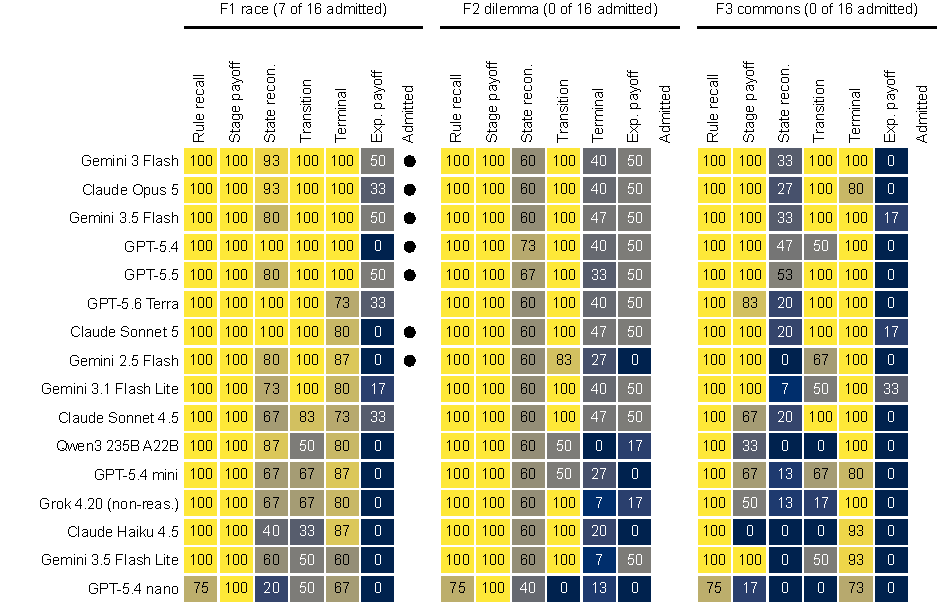
\includegraphics[width=\textwidth]{../../figures/arr/transfer_heatmap.pdf}
  \caption{Accuracy (\%) by domain for the 16 endpoints that completed all
  three families, ordered by F1 overall accuracy. A dot marks an admitted
  endpoint. The same thresholds admit seven of these endpoints on F1 and none
  on F2 or F3. Rule recall and stage payoff are near ceiling in every family;
  the families differ in state reconstruction and terminal scoring, the two
  gated domains.}
  \label{fig:heatmap}
\end{figure*}

\subsection{The name does not reproduce the verdict (C3)}
\label{sec:res-name}

On the original nine endpoints, the four refused endpoints were exactly the four
whose names contain \textit{mini}, \textit{nano} or \textit{lite}. With five
admitted of nine, the exact probability of that perfect agreement is 1/126.
If that held in general, the screen would cost sixty questions to read a
name.

It does not hold. Table~\ref{tab:baselines} gives the preregistered name rules
on the 17 endpoints that completed F1. The primary rule, refuse iff the name
has one of those three words, now agrees on 12 of 17, and five endpoints break
it: Claude Haiku 4.5, Claude Sonnet 4.5, GPT-5.6 Terra, Grok 4.20 and
Qwen3 235B are refused although their names carry no size word. A broader rule
that also treats \textit{haiku}, \textit{gemma} and the 20B open-weight model
as small agrees on 12 of 17 as well, now broken by that 20B model, which is
admitted with the highest F1 score of all (96.7\%). Both exact probabilities
are above 0.05 (0.053 and 0.088). The tie on nine endpoints was a property of
that roster.

Other free signals do no better. No single question reproduces the F1 verdict
on 17 endpoints: the best of the twenty, asked three times with a majority rule,
agrees on 14. On nine endpoints one question had reproduced it exactly, but
that question was found after the fact, and a question drawn at random agreed
on 5.8 of 9 on average. Format compliance runs the wrong way: on F1 the five
malformed answers all came from admitted endpoints, so requiring all sixty
answers to be well formed agrees with the verdict on 6 of 17.

\begin{table}[t]
  \centering
  \small
  \setlength{\tabcolsep}{4pt}
  \begin{tabular}{@{}lrr@{}}
    \toprule
    Rule for the F1 verdict & 9 endp. & 17 endp. \\
    \midrule
    Name has \textit{mini}/\textit{nano}/\textit{lite} & 9 & 12 \\
    \ \ exact $p$ of that agreement & 0.008 & 0.053 \\
    Broader size words & -- & 12 \\
    Best single question (majority of 3) & 9$^{\dagger}$ & 14 \\
    Median single question & 5 & 9 \\
    All answers well formed & -- & 6 \\
    State reconstruction $\geq$ 75\% alone & 9 & 15 \\
    Overall $\geq$ 80\% alone & 8 & 15 \\
    Refuse everyone & 4 & 9 \\
    \bottomrule
  \end{tabular}
  \caption{Agreement with the F1 verdict. $^{\dagger}$Found after inspecting
  the data; a randomly drawn question agreed on 5.8 of 9 on average. On 17
  endpoints no single question reproduces the verdict.}
  \label{tab:baselines}
\end{table}

\subsection{Rankings transfer, verdicts do not (C4)}
\label{sec:res-transfer}

Endpoints that do well on one game do well on the others.
Table~\ref{tab:transfer} gives the preregistered rank correlations over the 16
endpoints that completed all three families. On overall accuracy they range
from 0.66 to 0.87 and every interval excludes zero. On state reconstruction
alone they are weaker, 0.47 to 0.63, and the interval for F1 against F2 includes
zero (Figure~\ref{fig:scatter}). The reason is visible in the figure: on F2,
13 of 16 endpoints score exactly 60\% in state reconstruction, because they
answer the three counting questions and fail the two that sum six payoffs. A
domain that sits at one value cannot rank anything.

The verdicts do not transfer at all. At the same thresholds, F1 admits 8 of
17 endpoints, F2 admits 1 of 17 and F3 admits none of 16
(Figure~\ref{fig:heatmap}). Over the 16 common endpoints, F2 and F3 agree
on every verdict only because both refuse everyone, and F1 disagrees with both
on seven endpoints. The one endpoint admitted twice is the 20B open-weight
model, the only complete endpoint whose reasoning was switched on (a low
budget; Qwen3 received the same setting but is an instruct model without a
reasoning mode). It is also the only endpoint above half on expected payoff
(83\%). Under the preregistered decision rules, the name tie
is broken, so the screen carries information beyond the name; and the
state-reconstruction score does not transfer between F1 and F2, so a screen has
to be calibrated for the environment it gates.

\begin{table}[t]
  \centering
  \small
  \setlength{\tabcolsep}{3.5pt}
  \begin{tabular}{@{}lrrr@{}}
    \toprule
    & F1--F2 & F1--F3 & F2--F3 \\
    \midrule
    Overall & 0.66 & 0.87 & 0.83 \\
    \ \ 95\% CI & [0.28, 0.84] & [0.63, 0.95] & [0.52, 0.95] \\
    State recon. & 0.47 & 0.60 & 0.63 \\
    \ \ 95\% CI & [$-$0.05, 0.78] & [0.19, 0.85] & [0.32, 0.82] \\
    Same verdict & 9/16 & 9/16 & 16/16 \\
    \bottomrule
  \end{tabular}
  \caption{Spearman correlations between families over the 16 endpoints that
  completed all three, with bootstrap intervals over endpoints (10,000
  resamples). F2 and F3 admit nobody, so their agreement is total and
  uninformative, and Cohen's $\kappa$ is undefined.}
  \label{tab:transfer}
\end{table}

\begin{figure*}[t]
  \centering
  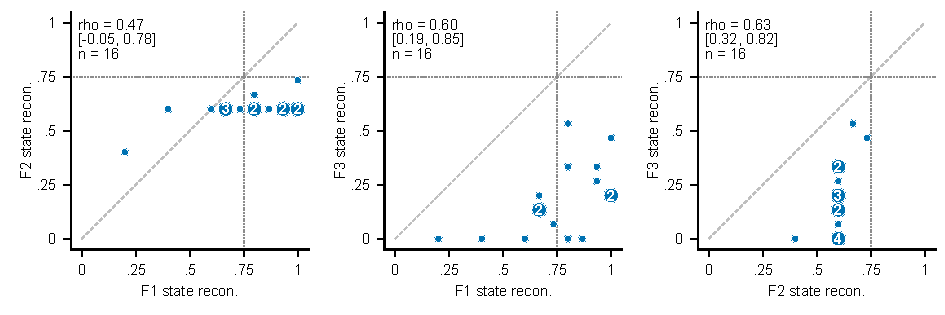
\includegraphics[width=\textwidth]{../../figures/arr/transfer_scatter.pdf}
  \caption{State-reconstruction accuracy for the 16 endpoints, family against
  family. Numbers inside markers count overlapping endpoints. Dotted lines mark
  the 75\% threshold. F2 piles up at 60\%, which caps the rank correlation it
  can show.}
  \label{fig:scatter}
\end{figure*}

\subsection{What makes a question hard}
\label{sec:res-items}

This analysis was not preregistered. We counted, for each of the 60
questions, how many values a correct answer has to combine: one for a recalled
rule or a single lookup, six for summing six payoffs, and so on, under a fixed
written rule (Appendix~\ref{sec:app-items}). Across the 60 questions that
count is strongly related to accuracy ($\rho=-0.74$, 95\% interval $-0.84$ to
$-0.59$), and the relation holds within each family ($-0.67$, $-0.75$ and
$-0.87$; Figure~\ref{fig:items}). The two F2 questions that sum six payoffs are
answered correctly on 4.2\% and 2.1\% of attempts; the answers are scattered
wrong totals, not a single misreading. The F3 questions that aggregate a
four-player table over four rounds fall to between 0\% and 37.5\%.

The count is not the whole story. Counting six defections is solved on every
attempt while summing six payoffs is almost never solved, so the operation
matters as well as the number of operands. What the pattern does show is that
under a one-shot answer with no room to work, longer arithmetic fails, and a
family's verdict depends on how much arithmetic its questions ask for. The one
endpoint that reasons before answering is the only one admitted on F2, which is consistent with
this reading but is one endpoint and not a test of it.

\begin{figure}[t]
  \centering
  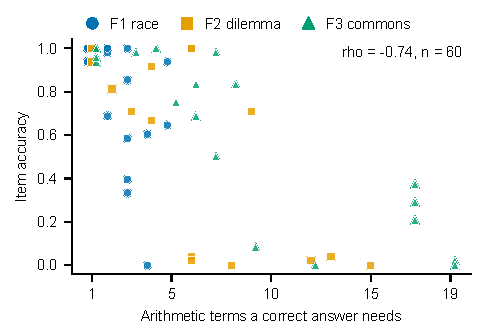
\includegraphics[width=\columnwidth]{../../figures/arr/item_load.pdf}
  \caption{Item accuracy against the number of values a correct answer
  combines, for all 60 questions, over the 16 common endpoints (48 answers per
  question). Exploratory.}
  \label{fig:items}
\end{figure}

\subsection{Agreement with the behaviour the screen gates}
\label{sec:res-behaviour}

The nine original endpoints also played the race game under one frozen
protocol, 30 games and 558 decisions each. How far an endpoint's play shifts
between the lowest and highest stated danger has a rank correlation of 0.87
with its F1 state-reconstruction score (exact $p=0.004$, $n=9$), and 0.77 with
its overall score. This is agreement between two measurements of the same nine
endpoints, not an estimated effect, and the screen does not partition the
behaviour: the highest-scoring refused endpoint shifts its play by 37.6 points
and the lowest-scoring admitted one by 38.2.

% =====================================================================
\section{Discussion}
\label{sec:discussion}

The screen passes the checks that are about the instrument and fails the one
that is about its use. It is repeatable, it is not a relabelled model name,
and its ranking of endpoints carries over to games with a different state. A
study that uses such a screen to describe which endpoints handle a game better
is on firm ground. A study that uses its absolute verdict as a statement that an
endpoint ``understood'' the game is not, because the same thresholds on
equivalent questions about similar games admit eight endpoints, one or none.

Four things are cheap to report and would let a reader judge a screen. First,
per-domain scores, since an aggregate hides which domain decides. Second, the
margin by which each admitted model clears each gate, beside the movement seen
on a repeat administration. Third, the free baselines: the name, one question,
format compliance and each gate alone, computed on the same data. Fourth, the
screen's items with their arithmetic load, or a second item set, so that a
verdict can be read as ``passed these questions'' rather than ``understood the
game''. Where a study must compare environments, relative standing or a
threshold calibrated per item set is safer than one fixed cut-off.

% =====================================================================
\section{Conclusion}
\label{sec:conclusion}

We treated a comprehension screen for language-model agents as an instrument
and tested it on three games and up to 17 endpoints under a preregistered plan.
It measures something real: it is repeatable, it is not a proxy for the name,
and its rankings transfer. Its verdict does not transfer, and the difficulty of
its questions, largely how much arithmetic they ask for, explains why. Who
passes a screen depends on the questions, and a study should say which
questions its agents passed.

\section*{Limitations}

The roster is 17 hosted endpoints from five providers on dates in September
2026; they are not a sample from a population of models, and endpoints can
change under a fixed name. Every rank statistic rests on $n\le17$. All three
families use one question wording per item and one output contract; paraphrase
and format effects are known to move scores \citep{mizrahi2024state,sclar2024quantifying}
and were not varied. The contract gives no room to reason before answering,
except for the one endpoint family that rejects a zero budget; a screen that
allowed working might give different verdicts, and our arithmetic-load account
is exploratory and rests on a hand-applied counting rule. Seven preregistered
endpoints produced no complete answers for reasons outside our control, which
narrows the roster in ways we did not choose. The behavioural agreement covers
nine endpoints in one game only.

\section*{Ethics Statement}

The study queries commercial language-model endpoints through a hosted
evaluation platform and involves no human participants; the first task family
is adapted from a published human experiment whose data we do not use. The
collection spread cells over several accounts of a hosted evaluation platform
under a plan fixed before collection; no account is named in the paper.

\bibliography{custom}

\appendix

\section{Probe Banks}
\label{sec:app-banks}

\paragraph{F2, iterated social dilemma.} Two players choose to cooperate or
defect each round with stage payoffs 3.2 (both cooperate), 0.4 and 4.7 (one
defects) and 1.3 (both defect). A player whose cooperation rate at the end is at
least 60\% receives a bonus of 7.5. State questions give four to six rounds of
play and ask for the opponent's defections, its last defection, either
player's accumulated payoff, or a cooperation rate.

\paragraph{F3, public goods.} Four players each receive 10 tokens a round and
contribute 0, 5 or 10; the pool is multiplied by 1.6 and shared equally. If the
group's contributions over the game reach 150, every player receives a bonus of
40. State questions give a four-round contribution table and ask for a
player's accumulated payoff, the group's average contribution, the number of
rounds above a level, or the distance to the target.

All three families share F1's stopping rule (at least five rounds, then a
20\% chance of stopping after each round) and its expected length of nine
rounds. Bank hashes (SHA-256, first 16 hex): F1 \texttt{2953fb472dcba475},
F2 \texttt{1cf954f988b379fb}, F3 \texttt{31ff7c47875bd700}. The full banks,
reference engines and tests are released with the code.

\section{Collection Failures}
\label{sec:app-failures}

\begin{table}[h]
  \centering
  \small
  \setlength{\tabcolsep}{3pt}
  \begin{tabular}{@{}lll@{}}
    \toprule
    Endpoint & Families & Failure \\
    \midrule
    Claude Opus 4.1 & all & unreachable (503) \\
    Claude Sonnet 4 & all & unreachable (503) \\
    Gemma 4 26B, 31B & all & no structured output \\
    GLM-5 & all & reasoning exhausts cap \\
    gpt-oss-120b & all & reasoning exhausts cap \\
    gpt-oss-20b & F3 & reasoning exhausts cap \\
    Gemini 2.5 Pro & none run & thinking mode only \\
    \bottomrule
  \end{tabular}
  \caption{Preregistered endpoints without a complete cell. Each transport
  failure was retried once on the same account, as preregistered.}
\end{table}

\section{Repeat Administrations of F1}
\label{sec:app-retest}

\begin{table}[h]
  \centering
  \small
  \setlength{\tabcolsep}{3pt}
  \begin{tabular}{@{}llrrl@{}}
    \toprule
    Endpoint & Cap & State & Overall & Verdict \\
    \midrule
    Claude Sonnet 5 & 128 &  86.7 & 76.7 & refused \\
                    & 256 &  86.7 & 81.7 & admitted \\
                    & 256 & 100.0 & 85.0 & admitted \\
    Gemini 3 Flash  & 128 & 100.0 & 95.0 & admitted \\
                    & 256 &  93.3 & 93.3 & admitted \\
                    & 256 &  93.3 & 93.3 & admitted \\
    Gemini 3.1 F.-Lite & 128 &  66.7 & 81.7 & refused \\
                    & 256 &  60.0 & 76.7 & refused \\
                    & 256 &  73.3 & 80.0 & refused \\
    GPT-5.4 nano    & 128 &  20.0 & 53.3 & refused \\
                    & 256 &  20.0 & 51.7 & refused \\
                    & 256 &  20.0 & 51.7 & refused \\
    \bottomrule
  \end{tabular}
  \caption{The four endpoints given F1 three times. The last two rows of each
  block differ in nothing recorded. One answer in state reconstruction is 6.7
  points.}
\end{table}

\section{Counting Rule for Item Load}
\label{sec:app-items}

A recalled rule or a single table lookup counts one. Counting occurrences in a
list of $k$ actions counts $k$. A rate's denominator counts one, as does a
threshold a computed value is compared with. Every constant that enters the
formula (prize, bonus, multiplier, maximum risk, expected length, stopping
probability, minimum rounds) counts one, and a value used twice counts once.
Scaling to a percentage is not counted. The count and a one-line justification
for every question are released with the code.

\end{document}
